%; whizzy chapter
% -initex iniptex -latex platex -format platex -bibtex jbibtex -fmt fmt
% 以上 whizzytex を使用する場合の設定。

%     Kansai Debian Meeting resources
%     Copyright (C) 2007 Takaya Yamashita
%     Thank you for Tokyo Debian Meeting resources

%     This program is free software; you can redistribute it and/or modify
%     it under the terms of the GNU General Public License as published by
%     the Free Software Foundation; either version 2 of the License, or
%     (at your option) any later version.

%     This program is distributed in the hope that it will be useful,
%     but WITHOUT ANY WARRANTY; without even the implied warranty of
%     MERCHANTABILITY or FITNESS FOR A PARTICULAR PURPOSE.  See the
%     GNU General Public License for more details.

%     You should have received a copy of the GNU General Public License
%     along with this program; if not, write to the Free Software
%     Foundation, Inc., 51 Franklin St, Fifth Floor, Boston, MA  02110-1301 USA

%  preview (shell-command (concat "evince " (replace-regexp-in-string "tex$" "pdf"(buffer-file-name)) "&"))
% 画像ファイルを処理するためにはebbを利用してboundingboxを作成。
%(shell-command "cd image200708; ebb *.png")

%%ここからヘッダ開始。

\documentclass[mingoth,a4paper]{jsarticle}
\usepackage{kansaimonthlyreport}
\usepackage[dvips]{xy}


% 日付を定義する、毎月変わります。
\newcommand{\debmtgyear}{2011}
\newcommand{\debmtgdate}{25}
\newcommand{\debmtgmonth}{12}
\newcommand{\debmtgnumber}{54}

\begin{document}

\begin{titlepage}

% 毎月変更する部分、本文の末尾も修正することをわすれずに

 第\debmtgnumber{}回 関西 Debian 勉強会資料

\vspace{2cm}

\begin{center}
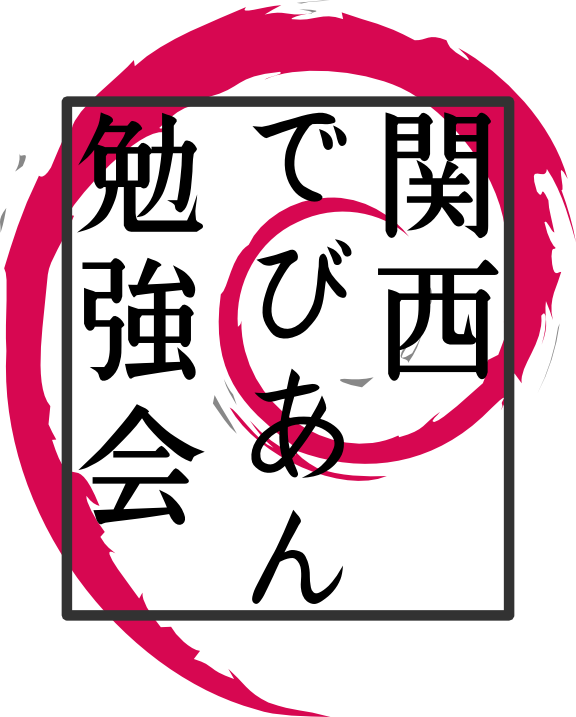
\includegraphics{image200802/kansaidebianlogo.png}
\end{center}

\begin{flushright}
\hfill{}関西 Debian 勉強会担当者 佐々木・倉敷・のがた・かわだ \\
\hfill{}\debmtgyear{}年\debmtgmonth{}月\debmtgdate{}日
\end{flushright}

\thispagestyle{empty}
\end{titlepage}

\dancersection{Introduction}{Debian JP}

 関西 Debian 勉強会はDebian GNU/Linux のさまざ
 まなトピック(新しいパッケージ、Debian 特有の機能の仕組、Debian 界隈で起
 こった出来事、などなど)について話し合う会です。

 目的として次の三つを考えています。
 \begin{itemize}
  \item MLや掲示板ではなく、直接顔を合わせる事での情報交換の促進
  \item 定期的に集まれる場所
  \item 資料の作成
 \end{itemize}

 それでは、楽しい一時をお楽しみ下さい。

\newpage

\begin{minipage}[b]{0.2\hsize}
 {\rotatebox{90}{\fontsize{80}{80}
{\gt 関西 Debian 勉強会}}}
\end{minipage}
\begin{minipage}[b]{0.8\hsize}
\hrule
\vspace{2mm}
\hrule
\setcounter{tocdepth}{1}
\tableofcontents
\vspace{2mm}
\hrule
\end{minipage}

\dancersection{最近のDebian関係のイベント報告}{Debian JP}

\subsection{第 53 回関西 Debian 勉強会}
53 回目の関西 Debian 勉強会は 2011 年 11 月 11 日(土)、12 日(日)に開催
された関西オープンソース 2011 にてブース出展とセッションをおこないまし
た。

ブースでは、Space Funデザインのポストカードが好評で多くの方に立ち寄って
いただけたようでした。東京からやまねさん、岩松さん、関西から木下さん、
矢吹さんが参加され DD の方々と交流を深めるよい機会になりました。

セッションでは、第 53 回関西 Debian 勉強会「なれる! Debian 開発者 ―
45 分でわかる?メンテナ入門」としてやまねさんによるメンテナのお仕事に
ついての発表がありました。質疑応答は活発で興味を持たれた方もおられるよ
うでした。

また、岩松さんによってGPG キーサインパーティと『Gitによるバージョン管
理』のサイン会も行われ、サイン会は開催前に本が売り切れるほど好評だった
ようです。

\subsection{第 82、83 回東京エリア Debian 勉強会}
82 回目の東京エリア Debian 勉強会は 2011 年 11 月 19 日(土)に開催された
オープンソースカンファレンス 2011 Tokyo/Fall にてブース出展とセッション
がおこなわれました。

83 回目の東京エリア Debian 勉強会は 2011 年 12 月 17 日(土)に開かれまし
た。
一年の振り返り、Debian GNU/kFreeBSD への porting の話、月刊 Debhelper
の発表があり、月刊 Debhelper は dh コマンドについて分かりやすい資料に
なっていますので興味のある方は資料\footnote{http://tokyodebian.alioth.debian.org/pdf/debianmeetingresume201112.pdf}
を参照してください。

\clearpage

\dancersection{事前課題}{Debian JP}

今回は以下の課題を出題しました.
\begin{screen}
  \begin{description}
  \item[事前課題1] Debian のパッケージで「バグを発見した、けど放置してい
    る」、もしくは Debian バグ追跡システムを探索してみて興味をもったバグ
    未解決パッケージがあれば挙げてください。
  \item[事前課題2] 関西Debian勉強会で今年印象に残った話と来年聞きたい話を
    教えてください。
  \item [事前課題3] 1月に予定している関西Debian勉強会温泉合宿に参加されま
    すか。
  \end{description}
\end{screen}

参加者の皆さんの解答は以下の通りです.

\begin{prework}{ 甲斐正三 }
  \begin{enumerate}
  \item 有りません。
  \item
    \begin{itemize}
    \item 最も印象に残った話: 第47回「ハッカーに一歩近づくTips vi編 」
      \begin{itemize}
      \item 理由1: vi(vim)は普段最もよく使っていてなじみがあるから。
      \item 理由2: 今まで使っていなかったが使うと便利なコマンドをいくつか使えるようになったから。''d100G'', ``y3G''など。
      \end{itemize}
    \item 来年聞きたい話:
      \begin{itemize}
      \item 「DebianにおけるARM Cortexとのいろいろ」
      \item Debianにおける新規CPUの開発環境構築
      \end{itemize}
    \end{itemize}
  \item 参加を希望します。
  \end{enumerate}
\end{prework}

\begin{prework}{ murase\_syuka }
  \begin{enumerate}
  \item Debian バグ追跡システムを探索方法が分からない。本番までに調べてみます。
  \item パッケージ作成とかの話。blender関連のパッケージ作りたい。
  \item 未定です。
  \end{enumerate}
\end{prework}

\begin{prework}{ 上川純一 }
  無回答。
\end{prework}

\begin{prework}{ 山下康成 }
  \begin{enumerate}
  \item なし \_o\_
  \item
    \begin{itemize}
    \item 今年印象に残った話: そりゃ、vi でしょ(笑
    \item 来年聞きたい話:
      Developer を増やすためにも、その底辺を広げる必要があるんじゃないでしょうか。
      Debian 入門編で新しい人を呼び込みませんか。
      \begin{itemize}
      \item Windows ユーザのためのDebian 入門
      \item Debian デスクトップ入門
      \item Debian インストールハンズオン
      \item Microsoft Office ユーザのための Libre Office 入門(Debian とは関係ないか...)
        \\ ...
      \end{itemize}
    \end{itemize}
  \item 残念ながら、ますます参加できなくなった感じ
  \end{enumerate}
\end{prework}

\begin{prework}{ 川江 }
  \begin{enumerate}
  \item バグではないけれど、KVMのVMの「音声」をDefaultで出るようにしてほしい。
  \item 来年はKVM関連の話が聞きたい。
  \item 参加できません。多分、San Franciscoに行ってると思います。
  \end{enumerate}
\end{prework}

\begin{prework}{ 門戸良介 }
  \begin{enumerate}
  \item すみません。ありません。
  \item
    今回初めての参加です。
    仕事で初めてLinuxを使い始めてはや3年になります。
    Linuxについてさらに理解を深めようと思い関西で参加できる勉強会としてDebianの勉強会に目をつけました。
    オープンソースへの造詣は浅いですが、好奇心は強いです。勉強会の雰囲気を感じ取って、出来れば継続的な参加をしていきたいと思っています。
  \item
    参加しません。
  \end{enumerate}
\end{prework}

\begin{prework}{ かわだてつたろう }
  \begin{enumerate}
  \item acpi-support: 0.138-10 に更新したらレジューム時にバックライトが点かなくなった。
  \item 運営の人になりました。
    bzr-buildpackage と git-buildpackage 話の内容とその時の会。
  \item 主催する人です。
  \end{enumerate}
\end{prework}

\begin{prework}{ kozo2 }
  \begin{enumerate}
  \item
    t-code(バグを発見した、けど放置している), alien(Debian バグ追跡システムを探索してみて興味をもったバグ未解決パッケージ)
  \item
    モダンな Debian パッケージ作成入門(関西Debian勉強会で今年印象に残った話), ライセンス系の話(来年聞きたい話)
  \item
    多分参加します。
  \end{enumerate}
\end{prework}

\begin{prework}{ のがたじゅん }
  \begin{enumerate}
  \item live-build 3.xでsyslinuxを使ってライブDVDを作った時、ファイル名が違うのでブートできない。
    パッチを書けばいいけど、マルチアーキの事もあるのでどう提案しようか考えたまま放置してましたが、ぼんやりこんな感じかなと思いついたので、正月にパッチを書こうかと思案中。
  \item
    ごめんなさい。今年はいろんな事があってあまり印象に残ってない…。
  \item
    考え中。温泉に行くまでが遠いので参加しないにちょっと傾きつつ…
  \end{enumerate}
\end{prework}

\begin{prework}{ 佐々木洋平 }
  \begin{enumerate}
  \item sid の rubygems が ruby1.8 で動きませぬ。yaml のパースが原因なんですが、どうしたら良いかなぁ、と数日放置しています。あと地味に痛いのは squeeze の elscreen が古いままで、コマンドラインからファイルを指定して Emacs を起動できません。sid のパッケージは直っているので backports すれば良いのですが、気力がなくて放置しています。…そういや\TeX Liveの2011への移行(+日本語対応)もあったな。
  \item Debian GNU/kFreeBSD の話(杉本さん)、IPv6のトンネル話(西山さん)、でしょうか。普段自分で触らないネタなので。
    来年は月間Debian Policyとか, DFSGから始めて月間FLOSSライセンスとか, 如何?
  \item いまのところ参加する気でおりまする。
  \end{enumerate}
\end{prework}

\begin{prework}{ lurdan }
  \begin{enumerate}
  \item squeeze 相当から sid に upgrade すると perl の migration に失敗する件。\#639290
  \item *-buildpackage の年だったかなぁとか。来年は月刊 debian policy なんてどうでしょう
  \item するする
  \end{enumerate}
\end{prework}

\begin{prework}{ よしだともひろ }
  \begin{enumerate}
  \item sip-testerというパッケージがIPv6リンクローカルアドレスに対応していないというバグ(もしかしたら仕様?)がありますが、放置中です。(動作可能なようとなるようなパッチは作りましたが)
  \item
    \begin{itemize}
    \item 今年印象に残った話: パッケージを作るのは実はそんなに難しくはないんだということ。
    \item 来年聞きたい話: 引き続いてパッケージ作成の話と、Debian開発者となるための道のりみたいな話が聞いてみたいです。
    \end{itemize}
  \item 残念ながら参加できそうにありません。
  \end{enumerate}
\end{prework}

\begin{prework}{ 金子真志 }
  \begin{enumerate}
  \item これまでは、本当に「使う」だけだったのでないです。今後は、もっと踏み込んで使ってDDになれるように頑張ります!!
  \item 今回初参加ですが、個人的なリクエストとして、「Debianパッケージの作り方〜ネットには載らないDebianDeveloper小技・テクニック〜」のような話を聞いてみたいです。(エディタのプラグインのおすすめとか・・・)
  \item 温泉合宿についてですが、学校の関係で参加したいですが、参加できなさそうです。
  \end{enumerate}
  今回初めての参加で、話についていけないかもしれませんが、これをきっかけにDebianについて学べればと思っています。
  どうぞよろしくお願いします.
\end{prework}

\begin{prework}{ Y.YATSUO }
  \begin{enumerate}
  \item wicd-gtk(1.7.1~b3)の翻訳がおかしい。BTS\#651804 upstreamで既に修正されてるっぽいです。
  \item パッケージング関連が充実してましたね
  \item 極力参加する方針で…
  \end{enumerate}
\end{prework}


\clearpage
\dancersection{さきが(ry NM 塾}{倉敷悟}

\subsection{NM とは何か}

Debian における NM (New Member) とは、新しく Debian Project の参加メンバーになった人、あるいは Debian Project に参加するための手続き、といった意味で使われます。後者の場合は、意味を明確にするために、NM プロセスといったりもします。
少し前までは、New Maintainer の略だったのですが、(パッケージ) メンテナ以外にも門戸を開こう、という方向性に変更されつつあります (とはいえ、現時点では NM プロセスはまだパッケージメンテナを念頭においた形のままです)。

\subsection{NMプロセスの紹介}

では、実際のNMプロセスを実例をもとにご紹介します。本当はもう少しプロセスを進めておくつもりだったのですが、あまりスムーズにいってないので途中までになっています。

NM 志願者向けのチェックリスト (http://www.debian.org/devel/join/nm-checklist) がありますので、まずはこれを見てみましょう。

\subsubsection{必要な条件}

まず、DD 2 名以上とキーサインしていること、さらに NM への応募を推薦してくれる DD が 1 名以上いること、これは具体的かつ最低限の条件になります。
加えて、すでに Debian に関わるある程度の活動をしてきていることも必要とされますが、これについては明確な線引きがあるわけではありませんし、今後変化してくる部分なので水物といっていいでしょう。

私の例だと、まともに Debian での活動をはじめたのは 2007 年くらいだったと思うので、おおよそ 4 年間、下積みとしてパッケージメンテ、翻訳、ローカルコミュニティ活動をしてきていますが、これはちょっと長かった (NM 応募が遅かった) かなぁ、と思っています。

最近では、DM のステップをふんでいることが推奨されていることもあるので、少なくとも6ヶ月以上特定のパッケージをメンテしていて、スポンサーと良好な関係を築けていれば、そのまま NM に進むことも可能でしょう。

\subsubsection{実例}

\begin{itemize}
\item 2011/11 (事前ネゴ)
\item 2011/12/04 apply
\item 2011/12/04 advocate checked by yyabuki
\item 2011/12/10 activity poll sent
\item 2011/12/11 pass frontdesk precheck
\item 2011/12/13 AM assigned to gwolf
\item 2011/12/16 AM assigned to laney
\item 2011/12/17 ID checked
\item 2011/12/25 (Philosophy and Procedure やりとり中)
\end{itemize}

この後に続く予定は、次のようになっています。

\begin{itemize}
\item Tasks and Skills
\item AM recommends to DAM
\item DAM Approval
\end{itemize}

\subsubsection{NMテンプレート}

NM 担当チームでは、主に AM 担当者向けの資料として、作業ガイドのリポジトリが用意しています(http://anonscm.debian.org/viewvc/nm/trunk/nm-templates/)。実は、ここを見れば、だいたい何を聞かれるのかはわかってしまいますので、予習のための参考書としては最良のものだと思われます。ただし、AM によっては NM テンプレートを使わない、という人もいますので、盲信はしすぎないようにしましょう。

\subsubsection{NM と 勉強会と Debian JP}

Debian 勉強会では、Debian Developer を育成する、を目的としてあげています。ですので、その運営主体である Debian JP としても、支援活動はいろいろとおこなわれています。具体的には、GPG キーサインの推進や、スポンサー探しのサポート、パッケージングスキルの教育、などです。是非有効に活用してください。

\subsubsection{NM と Debian Maintainer}

勉強会でも何度かとりあげていますが、いきなり NM は敷居が高い、という人のために、DM というステップが用意されています。これは、いわば「限定つきの Debian Developer」であり、スポンサーについてもらうことで自分のパッケージを Debian に含めることができる人達のことです。

事前の実績としてわかりやすいことや、内容がサブセットになっていることもあり、NM プロセスにおいても、事前に DM として活動しておくことが強く推奨されています。

\subsection{最後に}

\subsubsection{なぜ NM に?}

NM になることの意義を考えてみましょう。直接的には、次のようなメリットがあります。

\begin{itemize}
\item パッケージを自由にアップロードできる
\item LWN.net の購読権 (sponsored by HP)
\item Project Leader や GR への投票
\item @debian.org メールアカウント
\end{itemize}

あるいは若い人であれば、比較的名前の知られたプロジェクトへの参加自体や、プロジェクトに自分色を持ち込める、といった満足もあるかもしれません。
ただ、NM プロセスやその後の活動は、それなりに手間も気力も必要になります。これじゃ引きが足りない、という人も多いでしょう。

Debian 勉強会としては、前述したとおり、NM に応募しようと思える人材を育成したい、という思いがあるのですが、やはり動機の部分については、皆さんそれぞれの答えを見出していただくしかありません。

スライドの方では、一例として、特に技術的に秀でたものをもっているわけでもなく、業界的には定年に達してしまったおっさんが、一体何を考えて NM に挑戦してみているのか、簡単に紹介してみます。参考になれば。

\clearpage
\dancersection{t-code のバグレポをしてみた}{西田孝三}

\subsection{はじめに}

ここでは「Debianパッケージのバグを発見した場合にどうすればいいのか」を伝えることを目的とし、
実際のバグ例を挙げながらバグレポートの手順を説明します。
バグレポートするパッケージはEmacsで日本語入力するための拡張Elispであるt-codeパッケージです。
手順の大きな流れは下記の4段階に分けられます。

\begin{enumerate}
  \item バグトラッカーでの報告
  \item 自分で修正パッチを作る(可能であれば)
  \item 自分でDebianパッケージを作る(可能であれば)
  \item DebianDeveloper(DD)に3のパッケージを取り込んでもらう(知り合いのDDがいれば)
\end{enumerate}

実際にはまともにできたのは1だけでした。申し訳ありませんがお付き合いください。
それでは実際のt-codeパッケージのバグを見ながら順を追ってバグレポ、修正を行なっていきましょう。

\subsection{バグトラッカーでの報告}

t-codeのDebianパッケージは2003年のバージョン2.3.1以降更新がなくEmacs23や24で部首合成変換ができないバグがあります。
まずこのバグを報告する前にBug Trackerにすでに報告されていないかどうかウェブブラウザで簡単に確認しましょう。
DebianのBug TrackerのURLは http://www.debian.org/Bugs/ です。
バグの選択というselect boxとinput boxがありますのでそれぞれ「パッケージ名が」、「t-code」と入力しバグ報告情報を確認します。
2011年12月24日時点ではautomakeのバージョンに関するバグしか報告されていなかったので、バグ報告をする必要があることがわかりました。
reportbugというパッケージを用いると便利にバグ報告ができるため、もしこのパッケージがインストールされていなければインストールしてください。

\begin{commandline}
 $ sudo aptitude install reportbug
\end{commandline}

インストールができていればreportbugコマンドを入力します。

\begin{commandline}
kozo2@debian:~$ reportbug
Welcome to reportbug! Since it looks like this is the first time you have used reportbug, we are configuring its
 behavior. These settings will be saved to the file ``/home/kozo2/.reportbugrc'', which you will be
free to edit further.
Please choose the default operating mode for reportbug.

1 novice    Offer simple prompts, bypassing technical questions.

2 standard  Offer more extensive prompts, including asking about things that a moderately sophisticated user would
 be expected to know about Debian.

3 advanced  Like standard, but assumes you know a bit more about Debian, including ``incoming''.

4 expert    Bypass most handholding measures and preliminary triage routines. This mode should not be used by people
 unfamiliar with Debian's policies and operating procedures.

Select mode: [novice]
\end{commandline}

最初なので novice でいいと思います。

\begin{commandline}
Will reportbug often have direct Internet access? (You should answer yes to this question unless you know what you
 are doing and plan to check whether duplicate reports have been filed via some other channel.)
[Y|n|q|?]?
\end{commandline}

よくわからないので説明に従いYにします。

\begin{commandline}
What real name should be used for sending bug reports?
[kozo2]> Kozo Nishida
\end{commandline}

名前を入力します。

\begin{commandline}
Which of your email addresses should be used when sending bug reports? (Note that this address will be visible in
 the bug tracking system, so you may want to use a webmail address or another address with
spam filtering capabilities.)
[kozo2@debian]> knishida@riken.jp
\end{commandline}

メールアドレスを書きます。

\begin{commandline}
Do you have a ``mail transport agent'' (MTA) like Exim, Postfix or SSMTP configured on this computer to send mail
 to the Internet? [Y|n|q|?]? n
\end{commandline}

メールを送るプログラムの設定をしていなければnにします。

\begin{commandline}
Please enter the name of your SMTP host. Usually it's called something like ``mail.example.org'' or
 ``smtp.example.org''. If you need to use a different port than default, use the <host>:<port> alternative f
Just press ENTER if you don't have one or don't know, and so a Debian SMTP host will be used.
>
\end{commandline}

これもSMTP設定を知らないのでそのままENTERします。

\begin{commandline}
Please enter the name of your proxy server. It should only use this parameter if you are behind a firewall.
 The PROXY argument should be formatted as a valid HTTP URL, including (if necessary) a port num
example, http://192.168.1.1:3128/. Just press ENTER if you don't have one or don't know.
>
\end{commandline}

プロキシサーバも知らないのでそのままENTERします。

\begin{commandline}
Dear Maintainer,
*** Please consider answering these questions, where appropriate ***

   * What led up to the situation?
   * What exactly did you do (or not do) that was effective (or
     ineffective)?
   * What was the outcome of this action?
   * What outcome did you expect instead?

*** End of the template - remove these lines ***


-- System Information:
Debian Release: wheezy/sid
  APT prefers unstable
  APT policy: (500, 'unstable')
Architecture: amd64 (x86_64)

Kernel: Linux 3.1.0-1-amd64 (SMP w/2 CPU cores)
Locale: LANG=ja_JP.UTF-8, LC_CTYPE=ja_JP.UTF-8 (charmap=UTF-8)
Shell: /bin/sh linked to /bin/dash

Versions of packages t-code depends on:
ii  emacs-snapshot-nox [emacs-snapshot]  1:20111219-1

t-code recommends no packages.

t-code suggests no packages.

-- no debconf information
\end{commandline}

こういうひな形が表示されますのでこれを編集します。
以下が編集後のレポートです。

\begin{commandline}
Subject: t-code version 2.3.1 fails bushu-convert
Package: t-code
Version: 2:2.3.1-3
Severity: normal

Dear Maintainer,
*** Please consider answering these questions, where appropriate ***

   * T-code pre bushu-convert doesn't work
   * pre bushu-convert error message is tcode-self-insert-command: Wrong type argument: characterp, nil
   * T-code post bushu-convert doesn't work(There is no error message).

-- System Information:
Debian Release: wheezy/sid
  APT prefers unstable
  APT policy: (500, 'unstable')
Architecture: amd64 (x86_64)

Kernel: Linux 3.1.0-1-amd64 (SMP w/2 CPU cores)
Locale: LANG=ja_JP.UTF-8, LC_CTYPE=ja_JP.UTF-8 (charmap=UTF-8)
Shell: /bin/sh linked to /bin/dash

Versions of packages t-code depends on:
ii  emacs-snapshot-nox [emacs-snapshot]  1:20111219-1

t-code recommends no packages.

t-code suggests no packages.

-- no debconf information
\end{commandline}

ま、こんなとこでしょう。
編集を終えると下記の確認をしてきます。

\begin{commandline}
Report will be sent to ``Debian Bug Tracking System'' <submit@bugs.debian.org>''--configure'' option.
Submit this report on t-code (e to edit) [Y|n|a|c|e|i|l|m|p|q|d|t|s|?]? Y
\end{commandline}

これでよいのでYを入力します。もう一度編集したければeを入力します。

\begin{commandline}
Connecting to reportbug.debian.org via SMTP...

Bug report submitted to: ``Debian Bug Tracking System'' <submit@bugs.debian.org>
Copies will be sent after processing to:
  knishida@riken.jp

If you want to provide additional information, please wait to receive the bug tracking number via email;
 you may then send any extra information to n@bugs.debian.org (e.g. 999999@bugs.debian.org), where n is the
bug number. Normally you will receive an acknowledgement via email including the bug report number within
 an hour; if you haven't received a confirmation, then the bug reporting process failed at some point
(reportbug or MTA failure, BTS maintenance, etc.).
\end{commandline}

これでバグレポートは終わりです。
入力した自分のメールアドレスにバグレポートしたことを確認するメールが届いていることを確認してください。
もしメールが届いていたらバグレポートの番号を確認して
http://bugs.debian.org/cgi-bin/bugreport.cgi?bug=653167
のようにbug=の後にバグIDを入力してウェブページでも内容を確認してみてください。

\subsection{自分で修正パッチを作る}

もし可能であればDebianのルールに従い修正パッチを作ってみましょう。
t-codeは安宅正之さんが中心となりGoogle codeで開発を引き継がれており(http://code.google.com/p/tcode/)、このリポジトリのtrunkのt-codeはEmacs23、24で使えることを確認しています。
また青田直大さんが個人的に修正をされたgithubのリポジトリ(https://github.com/naota/tc)もEmacs23,24で使えることを確認しています。

どちらのリポジトリのコードをどのようにパッケージ化していけばよいか(これまでのコードとの差分情報の記述など)わからなかったためこの部分については次回への宿題ということにさせてください。
申し訳ありません。
と、いうわけで次回は「バグ修正リポジトリコードの取り込みとdpatchの使い方」で発表させてください。

\subsection{自分でDebianパッケージを作る}

本来ならこれまでのパッケージからの変更をDebianのルールに従って記述したファイルを作成する必要があるかと思いますが、ここではその手続をすっとばして
前述のリポジトリのソースコードの内、安宅さんのリポジトリのソースコードを用いてDebianパッケージを作ることを試みます。

まずt-codeパッケージのソースコードを取得します。

\begin{commandline}
$ apt-get source t-code
$ svn checkout http://tcode.googlecode.com/svn/trunk/ tcode-read-only
$ ls
t-code-2.3.1  t-code_2.3.1-3.diff.gz  t-code_2.3.1-3.dsc  t-code_2.3.1.orig.tar.gz
\end{commandline}

次にソース中のdebianディレクトリを安宅さんのリポジトリのソースコード中にコピーします。

\begin{commandline}
$ cp -r t-code-2.3.1/debian tcode-read-only/tc/
\end{commandline}

それではこれでDebian packageが作れるか試してみましょう。
Debian packageはdebuildコマンドで作成できます。
debuildコマンドはdevscriptsパッケージをインストールすると使えるようになります。

\begin{commandline}
$ sudo aptitude install devscripts
$ cd tcode-read-only/tc
$ sudo debuild -us -uc
This package has a Debian revision number but there does not seem to be
an appropriate original tar file or .orig directory in the parent directory;
(expected one of t-code_2.3.1.orig.tar.gz, t-code_2.3.1.orig.tar.bz2,
t-code_2.3.1.orig.tar.lzma,  t-code_2.3.1.orig.tar.xz or tc.orig)
continue anyway? (y/n) y
\end{commandline}

親ディレクトリにソースのtar.gzがないと言われますが無視してbuildを試みます。

\begin{commandline}
make[2]: `install-exec-am' に対して行うべき事はありません.
/bin/sh ../mkinstalldirs /home/kozo2/tcode-read-only/tc/debian/t-code/usr/share/tc
 /usr/bin/install -c -m 644 ./pd_kihon.yom /home/kozo2/tcode-read-only/tc/debian/t-code/usr/share/tc/pd_kihon.yom
 /usr/bin/install -c -m 644 ./greece.maz /home/kozo2/tcode-read-only/tc/debian/t-code/usr/share/tc/greece.maz
 /usr/bin/install -c -m 644 ./jukujiku.maz /home/kozo2/tcode-read-only/tc/debian/t-code/usr/share/tc/jukujiku.maz
 /usr/bin/install -c -m 644 ./t225.dat /home/kozo2/tcode-read-only/tc/debian/t-code/usr/share/tc/t225.dat
 /usr/bin/install -c -m 644 ./t300.dat /home/kozo2/tcode-read-only/tc/debian/t-code/usr/share/tc/t300.dat
 /usr/bin/install -c -m 644 ./t400.dat /home/kozo2/tcode-read-only/tc/debian/t-code/usr/share/tc/t400.dat
 /usr/bin/install -c -m 644 ./t450.dat /home/kozo2/tcode-read-only/tc/debian/t-code/usr/share/tc/t450.dat
 /usr/bin/install -c -m 644 ./t575.dat /home/kozo2/tcode-read-only/tc/debian/t-code/usr/share/tc/t575.dat
 /usr/bin/install -c -m 644 ./t675.dat /home/kozo2/tcode-read-only/tc/debian/t-code/usr/share/tc/t675.dat
 /usr/bin/install -c -m 644 ./t900.dat /home/kozo2/tcode-read-only/tc/debian/t-code/usr/share/tc/t900.dat
 /usr/bin/install -c -m 644 ./t1200.dat /home/kozo2/tcode-read-only/tc/debian/t-code/usr/share/tc/t1200.dat
 /usr/bin/install -c -m 644 ./t1353.dat /home/kozo2/tcode-read-only/tc/debian/t-code/usr/share/tc/t1353.dat
 /usr/bin/install -c -m 644 ./itaiji.maz /home/kozo2/tcode-read-only/tc/debian/t-code/usr/share/tc/itaiji.maz
 /usr/bin/install -c -m 644 ./mazegaki.dic /home/kozo2/tcode-read-only/tc/debian/t-code/usr/share/tc/mazegaki.dic
 /usr/bin/install -c -m 644 ./mkcertain.pl /home/kozo2/tcode-read-only/tc/debian/t-code/usr/share/tc/mkcertain.pl
make[2]: ディレクトリ `/home/kozo2/tcode-read-only/tc/mazegaki' から出ます
make[1]: ディレクトリ `/home/kozo2/tcode-read-only/tc/mazegaki' から出ます
/usr/bin/make -C skkinput3  DESTDIR=/home/kozo2/tcode-read-only/tc/debian/t-code install
make[1]: ディレクトリ `/home/kozo2/tcode-read-only/tc/skkinput3' に入ります
make[2]: ディレクトリ `/home/kozo2/tcode-read-only/tc/skkinput3' に入ります
/bin/sh ../mkinstalldirs /home/kozo2/tcode-read-only/tc/debian/t-code/usr/bin
mkdir /home/kozo2/tcode-read-only/tc/debian/t-code/usr/bin
 /usr/bin/install -c tcinput /home/kozo2/tcode-read-only/tc/debian/t-code/usr/bin/tcinput
/bin/sh ../mkinstalldirs /home/kozo2/tcode-read-only/tc/debian/t-code/usr/share/tc
 /usr/bin/install -c -m 644 ./init.el /home/kozo2/tcode-read-only/tc/debian/t-code/usr/share/tc/init.el
 /usr/bin/install -c -m 644 ./skk-startup.el /home/kozo2/tcode-read-only/tc/debian/t-code/usr/share/tc/skk-startup.el
 /usr/bin/install -c -m 644 ./tc-skki.el /home/kozo2/tcode-read-only/tc/debian/t-code/usr/share/tc/tc-skki.el
 /usr/bin/install -c -m 644 ./load-path.el /home/kozo2/tcode-read-only/tc/debian/t-code/usr/share/tc/load-path.el
make[2]: ディレクトリ `/home/kozo2/tcode-read-only/tc/skkinput3' から出ます
make[1]: ディレクトリ `/home/kozo2/tcode-read-only/tc/skkinput3' から出ます
cd /home/kozo2/tcode-read-only/tc/debian/t-code/usr/share/t-code && \
                chmod +x bushu2canna where mkcertain.pl
/bin/sh: 1: cd: can't cd to /home/kozo2/tcode-read-only/tc/debian/t-code/usr/share/t-code
make: *** [install] エラー 2
dpkg-buildpackage: error: fakeroot debian/rules binary gave error exit status 2
debuild: fatal error at line 1348:
dpkg-buildpackage -rfakeroot -D -us -uc failed
\end{commandline}

失敗でした!
今回はここまででお許しください。パッケージ作成成功は次回の発表までの宿題ということで!

\subsection{DDにパッケージをDebianのリポジトリに取り込んでもらう}

Debianパッケージができたら、関西のDDにビールでも飲みながら話しかけてみましょう。

\subsection{おわりに}

おもいっきり尻切れトンボで申し訳ありません!
ただ、最初のバグレポートをするだけでもそれはそれで結構Debianに貢献していることになると思います。
何事も最初のとっかかりさえ掴めれば後は楽かと思いますので皆さんもどんどんバグ報告をして残りのパッチ作成や、パッケージ作成も一緒にやってみませんか。
それではまた次回!(土下座)

\clearpage
\dancersection{2011年の振り返りと2012年の企画}{Debian JP}

今月が2011年最後の関西Debian勉強会になります。初回が2007年3月なので、今年で5年目になりますね。

\subsection{勉強会全体}

毎回のセッションについてですが、
今年はパッケージ作成やBTSに関する題材が多く扱われました。
定番のネタ(Debianの入門的なお話、ライセンス、パッケージ作成、BTS)などの題材は
毎年更新されていくべき題材なので, 今後も繰り返し扱っていきたい所です。
事前課題で提出されていた「インストール大会」のような初心者講習もやってみたい
所ですね。

また、昨年から事前課題の提出が普通になってきましたので、
来年からは事後統計(アンケート)も提出してもらおうか, なんて考えています。

運営に関しては、常連さんだった河田さんが運営側になり、Debian JP Project
へ加入されました。また、今回の発表にある通り倉敷さんが DD になるため
の NM プロセスへ申請されています。

イベント参加については、OSC Kansai@ Kobe, OSC Hokkaido, OSC Kansai@
Kyoto, KOF に参加しました。勉強会から fork した GPG キーサインパーティも
毎回実施されています。今後も継続して参加する予定です。

\subsection{開催実績}

関西Debian勉強会の出席状況を確認してみましょう。グラフで見る
と\fgref{fig:kansaipeoplechart}になります。また、毎回の参加者の人数とその
際のトピックを \tbref{tab:count2011kansai} にまとめました。グラフ中の黒線
は参加人数, 赤線は1年の移動平均です。参加人数が$0$となっているところは人
数が集計されていないor開催されなかった月ですので、欠損値処理をした方が良いですね%
\footnote{R使った事ないので今日は間に合いませんでした}。

Debian勉強会申し込みシステムを使用するようになり, 事前課題を設定すること
も多くなりました。また, アンケートシステムも稼動するようになるでしょうか
ら、今後は事前課題と事後課題のグラフを追加しようと思っています。


\begin{figure}[h]
  \begin{center}
    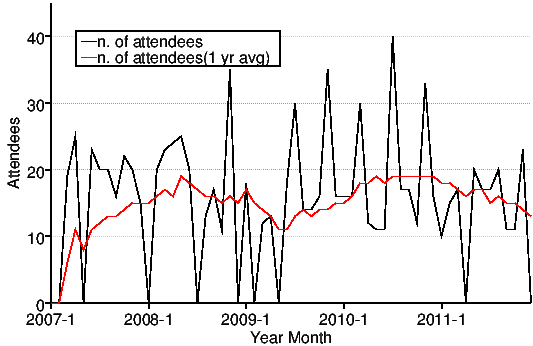
\includegraphics[width=.8\hsize]{image201112/memberanalysis/kansai.png}
  \end{center}
  \caption{関西の参加人数推移(参加人数と12ヶ月移動平均)}
  \label{fig:kansaipeoplechart}
\end{figure}
\begin{table}
  \begin{minipage}{0.5\hsize}
    \caption{関西Debian勉強会の参加人数とトピック(2007年)}
    \begin{center}
      \begin{tabular}{|l|c|p{10em}|}
        \hline
                   & 参加人数 & 内容 \\
        \hline
        2007年3月  & 19       & 開催にあたり \\
        2007年4月  & 25       & goodbye、youtube、プロジェクトトラッカー\\
        2007年6月  & 23       & 社会契約、テーマ、debian/rules、bugreport\\
        2007年7月  & 20前後   & OSC-Kansai \\
        2007年8月  & 20       & Inkscape、patch、dpatch\\
        2007年9月  & 16       & ライブラリ、翻訳、debtorrent\\
        2007年10月 & 22       & 日本語入力、SPAMフィルタ\\
        2007年11月 & 20前後   & KOF \\
        2007年12月 & 15       & 忘年会、iPod touch\\
        \hline
      \end{tabular}
    \end{center}
  \end{minipage}
  \begin{minipage}{0.45\hsize}
    \begin{center}
    \caption{関西Debian勉強会参加人数(2008年)}\label{tab:count2008kansai}
    \vspace{-1em}
      \begin{tabular}{|l|c|p{10em}|}
        \hline
                   & 参加人数 & 内容 \\
        \hline
        2008年2月  & 20       & PC Cluster, GIS, \TeX \\
        2008年3月  & 23       & bug report, developer corner, GPG \\
        2008年4月  & 24       & coLinux, Debian GNU/kFreeBSD, sid \\
        2008年5月  & 25       & ipv6, emacs, ustream.tv\\
        2008年6月  & 20       & pbuilder, hotplug, ssl\\
        2008年8月  & 13       & coLinux \\
        2008年9月  & 17       & debian mentors, ubiquity, DFSG\\
        2008年10月 & 11       & cdbs,cdn.debian.or.jp \\
        2008年11月 & 35       & KOF \\
        2008年12月 & ?        & TeX資料作成ハンズオン\\
        \hline
      \end{tabular}
    \end{center}
  \end{minipage}
\end{table}
\begin{table}
  \begin{minipage}{0.5\hsize}
%    \begin{table}
    \caption{関西Debian勉強会の参加人数とトピック(2009-2010)}
    % \caption{関西Debian勉強会参加人数(2009)}\label{tab:count2009kansai}
    \begin{center}
      \begin{tabular}{|l|c|p{10em}|}
        \hline
                   & 参加人数 & 内容 \\
        \hline
        2009年1月  & 18       & DMCK, LT \\
        2009年3月  & 12       & Git \\
        2009年4月  & 13       & Installing sid, Mancoosi, keysign \\
        2009年6月  & 18       & Debian Live, bash\\
        2009年7月  & 30?      & OSC2009Kansai \\
        2009年8月  & 14       & DDTSS, lintian \\
        2009年9月  & 14       & reportbug, debian mentors\\
        2009年10月 & 16       & gdb, packaging \\
        2009年11月 & 35       & KOF2009 \\
        2009年12月 & 16       & GPS program, OpenStreetMap \\
        \hline
  %     \end{tabular}
  %   \end{center}
  % \end{minipage}
  % \begin{minipage}{0.5\hsize}
  %   \caption{関西Debian勉強会参加人数(2010年)}\label{tab:count2010kansai}
  %   \begin{center}
  %     \begin{tabular}{|l|c|p{10em}|}
        \hline
                   & 参加人数 & 内容 \\
        \hline
        2010年1月  & 16       & Xen, 2010年企画 \\
        2010年2月  & 16       & レンタルサーバでの利用, GAE \\
        2010年3月  & 30?      & OSC2010Kobe \\
        2010年4月  & 12       & デスクトップ環境, 正規表現 \\
        2010年5月  & 11       & ubuntu, squeeze \\
        2010年6月  & 11       & debhelper7, cdbs, puppet \\
        2010年7月  & 40?      & OSC2010Kyoto \\
        2010年8月  & 17       & emdebian, kFreeBSD \\
        2010年9月  & 17       & タイルWM \\
        2010年10月 & 12       & initramfs, debian live \\
        2010年11月 & 33       & KOF2010 \\
        2010年12月 & 14       & Proxmox, annual review \\
        \hline
      \end{tabular}
    \end{center}
  \end{minipage}
% \end{table}
% \begin{table}
  \begin{minipage}{.45\linewidth}
    \caption{関西Debian勉強会の参加人数とトピック(2011)}\label{tab:count2011kansai}
    \begin{center}
      \begin{tabular}{|l|c|p{10em}|}
        \hline
        開催年月  & 参加人数 & 内容 \\
        \hline
        2011年1月 &10        & BTS, Debian GNU/kFreeBSD\\
        2011年2月 &15        & pbuilder, Squeezeリリースパーティ\\
        2011年3月 &17        & ライセンス, Debianのドキュメント関連\\
        2011年4月 &25        & OSC 2011 Kansai @ Kobe, GPG キーサインパーティ \\
        2011年5月 &20        & vi, dpkg \\
        2011年6月 &17        & IPv6, vcs-buildpackage{svn, git}\\
        2011年7月 &17        & OSC 2011 Kansai @ Kyoto, GPG キーサインパーティ\\
        2011年8月 &20        & Debianパッケージ作成ハンズオン\\
        2011年9月 &11        & vcs-buildpackage{bzr, git}\\
        2011年10月&11        & Emacs, vim の拡張のDebianパッケージ, 翻訳\\
        2011年11月&23        & KOF 2011\\
        2011年12月&13        & NMプロセス, BTS\\
        \hline
      \end{tabular}
    \end{center}
  \end{minipage}
\end{table}



\clearpage
\dancersection{今後の予定}{Debian JP}

\subsection{次回}
次回は、2012年1月28、29日の二日間にいつもと趣きを変えて京都の湯の花温泉
にて Debian 温泉合宿を行います。

次々回は、2012年2月26日に福島区民センターでいつも通りの勉強会を行います。
発表については未定ですので、みなさまの発表をお待ちしております。

% 冊子にするために、4の倍数にする必要がある。
% そのための調整
% \dancersection{メモ}{}
% \mbox{}\newpage
% \mbox{}\newpage

\printindex
 \cleartooddpage

 \begin{minipage}[b]{0.2\hsize}
  \rotatebox{90}{\fontsize{80}{80} {\gt 関西 Debian 勉強会} }
 \end{minipage}
 \begin{minipage}[b]{0.8\hsize}

 \vspace*{15cm}
 \rule{\hsize}{1mm}
 \vspace{2mm}
 
\includegraphics[width=2cm]{image200502/openlogo-nd.eps}
 \noindent \Large \bf Debian 勉強会資料\\ \\
 \noindent \normalfont \debmtgyear{}年\debmtgmonth{}月\debmtgdate{}日 \hspace{5mm}  初版第1刷発行\\
 \noindent \normalfont 関西 Debian 勉強会 (編集・印刷・発行)\\
 \rule{\hsize}{1mm}
 \end{minipage}

\end{document}
